\section{Hybrid Perspectives and Future Memory Hierarchies}

Hybrid memory hierarchies aim to combine the high speed of DRAM with the non-volatility of FeRAM (including FeFET variants). By placing FeRAM close to DRAM or the memory controller, systems can reduce refresh energy, enable instant-on functionality, and support fast checkpointing and recovery.

\subsection*{Benefits}
\begin{itemize}
  \item \textbf{Reduced refresh overhead:} Part of the dataset can be parked in FeRAM, cutting DRAM refresh traffic and standby power.
  \item \textbf{Fast persistence:} System state can be checkpointed to FeRAM with microsecond-scale latency, enabling quick resume.
  \item \textbf{Data resilience:} FeRAM provides crash consistency for critical metadata and write-back buffers.
\end{itemize}

\subsection*{Constraints and trade-offs}
\begin{itemize}
  \item \textbf{Endurance and variability:} FeRAM endurance ($10^{12}$--$10^{13}$ cycles) is high but still below DRAM refresh activity; device variability must be managed.
  \item \textbf{Write energy and latency:} FeRAM generally incurs higher write energy than DRAM; policies should bias read-mostly or cold data to FeRAM.
  \item \textbf{Integration cost:} Adopting FeFET or ferroelectric layers in advanced CMOS nodes introduces process-compatibility and reliability risks (e.g., TDDB under high fields).
\end{itemize}

\subsection*{System design directions}
\begin{itemize}
  \item \textbf{Tiering policies:} Classify pages/objects by write intensity and retention needs, migrating cold or persistent data to FeRAM.
  \item \textbf{Refresh co-optimization:} Dynamically shrink DRAM refresh for regions shadowed or backed by FeRAM.
  \item \textbf{Checkpoint and logging:} Exploit FeRAM bandwidth for low-latency state persistence.
  \item \textbf{Controller support:} Maintain metadata for wear leveling, retention-aware placement, and error monitoring (e.g., soft/hard failure counters).
\end{itemize}

\begin{figure}[!t]
\centering
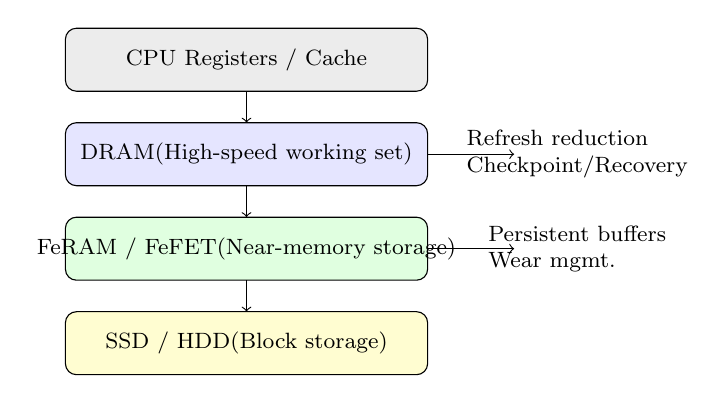
\begin{tikzpicture}[font=\footnotesize]
  \draw[fill=gray!15, rounded corners] (-2.3,3.0) rectangle (2.3,3.8);
  \node at (0,3.4) {CPU Registers / Cache};

  \draw[fill=blue!10, rounded corners] (-2.3,1.8) rectangle (2.3,2.6);
  \node at (0,2.2) {DRAM\\(High-speed working set)};

  \draw[fill=green!12, rounded corners] (-2.3,0.6) rectangle (2.3,1.4);
  \node at (0,1.0) {FeRAM / FeFET\\(Near-memory storage)};

  \draw[fill=yellow!18, rounded corners] (-2.3,-0.6) rectangle (2.3,0.2);
  \node at (0,-0.2) {SSD / HDD\\(Block storage)};

  \draw[->] (0,3.0) -- (0,2.6);
  \draw[->] (0,1.8) -- (0,1.4);
  \draw[->] (0,0.6) -- (0,0.2);

  \node[align=left] at (4.2,2.2) {Refresh reduction\\Checkpoint/Recovery};
  \node[align=left] at (4.2,1.0) {Persistent buffers\\Wear mgmt.};
  \draw[->] (2.3,2.2) -- (3.4,2.2);
  \draw[->] (2.3,1.0) -- (3.4,1.0);
\end{tikzpicture}
\caption{Hybrid memory hierarchy integrating DRAM and FeRAM (near-memory).}
\label{fig:hybrid_hierarchy}
\end{figure}
